\section{Structure}\label{sec:Structure}
For the simulation environment to be useful some basic functionality is needed. The simulation should be easy to setup and adjust if needed. 
Furthermore an easy way to view the result of the simulation is needed such that necessary adjustments can easily be made based on the result.

The first overall thing to consider is the composition of components desired to simulate. 
To make the simulation environment useful it should be able to handle different compositions of pipes and tanks. Meaning that the simulation environment can simulate different setups than the one shown in figure \ref{fig:kloakgrid_simplified}. For this a simple setup procedure, where different sizes of pipes with different parameters can be chosen, is needed. 
The second thing to consider is that the environment should be brought to a steady state before the simulation starts. The reason for this is that unintended results can arise when working with non-linear systems. Also if a linearized approach to the MPC scheme is chosen a linearized model is necessary, which requires a system in steady state to obtain. 
The simulation should be able to run for a predefined amount of iterations. 
Based on this the basic structure of the simulation environment can be split in to three parts as shown in figure \ref{fig:struct_overview}.

\begin{figure}[H]
\centering
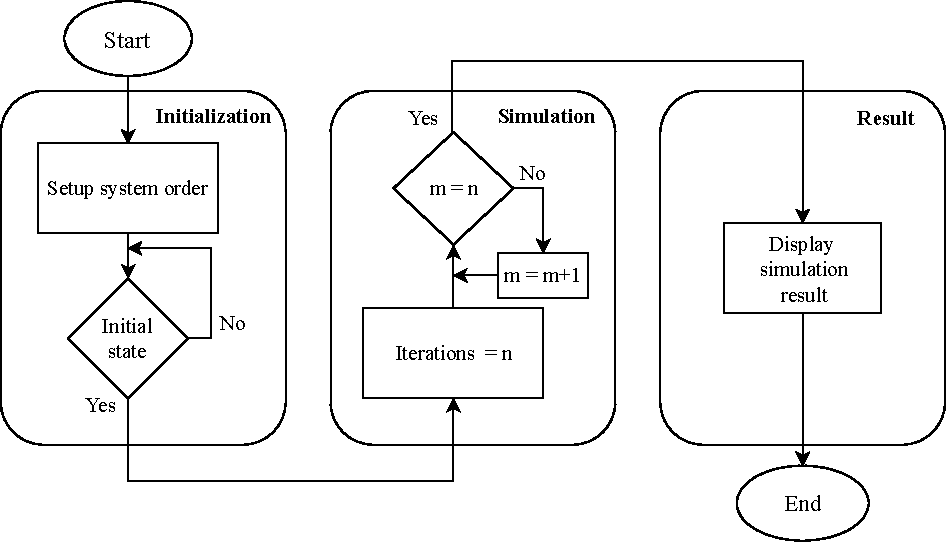
\includegraphics[width=0.9 \textwidth]{report/simulation/pictures/struct_overview.pdf}
\caption{Basic overview of simulation environment}
\label{fig:struct_overview}
\end{figure}


% \begin{enumerate}
% 	\item Initialization
% 	\item Simulation
% 	\item Result
% \end{enumerate}

%To solve the non-linear equations obtained for the free flow channel model in subsection \ref{subse:open_channel} the Preissman scheme is utilized. This scheme is explained in detail in section 
The following will go into details of the design off, and the considerations made during the design phase, of the three part shown in the figure.

\subsection*{Initialization} 
The initialization process is as shown in figure \ref{fig:struct_overview} comprised of several parts. The first part is to setup the desired system of pipes and tanks such that the system is simulated with the chosen components in the right order.
%As mentioned in section \ref{ch:simulation_solution_and_limitation} a solution to minimize flow and concentrate variations could be insertion of one or more tanks in the sewer network. 
Secondly the system should be brought in to a steady state from which the simulation can start.
The reason for this is that the Saint-Venant equations utilized to simulate the flow in the sewer pipes is non-linear. Because of this it can be difficult to find a steady state by hand which do not produce a unintended result when starting simulating. Though it might be possible to find fitting initial values for small setup the assumptions is that a larger setup will increase the chance of unintended results when starting simulating.

For the first part a simple system setup, consisting of a MATLAB function is decided upon. The order of the components in the function decides the place to be in the system when simulating. An example of this the setup procedure is shown in figure \ref{fig:sys_setup}  

\begin{figure}[H]
\centering
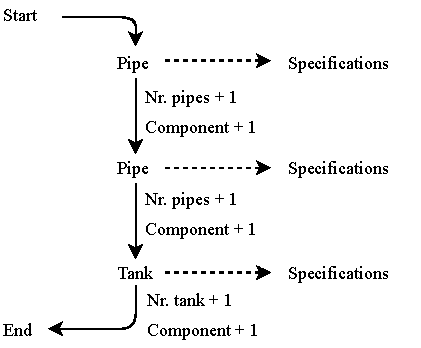
\includegraphics[width=0.55 \textwidth]{report/simulation/pictures/sys_setup.pdf}
\caption{Setup scheme of system order initiation}
\label{fig:sys_setup}
\end{figure}

The specifications for each part in figure \ref{fig:sys_setup} refers to the parameters needed to run the simulation by the 
The necessary specifications entered for pipe and tank should as a minimum be the required parameters needed to utilize the Preissmann scheme explained in section \ref{se:preissmann_scheme} and to simulate in- and outflow of one or more tanks, respectively. Furthermore constants which is utilized during simulation should be calculated during initialization such that the computational load is kept as low as possible during simulation. 

A simple solution to bring the desired system setup to an initial steady state is to give a fixed input flow and iterate. 
The iteration continues until a satisfactory error between the fixed input and the flow within the designated setup is deemed sufficiently low. For this to work it is important to have side input or disturbance input in mind. In figure \ref{fig:simple_sewer} a simple setup is shown of a possible setup to be simulated. 

\begin{figure}[H]
\centering
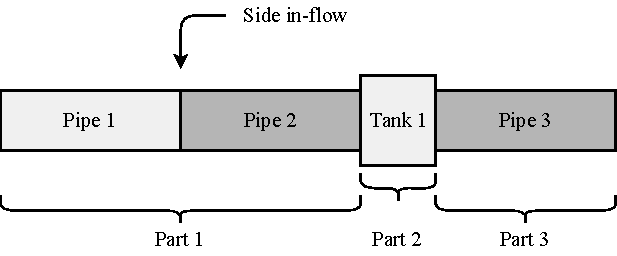
\includegraphics[width=0.55 \textwidth]{report/simulation/pictures/simple_sewer.pdf}
\caption{Simple setup with three pipes, a tank and a single side input}
\label{fig:simple_sewer}
\end{figure}

To make the steady state iteration scheme work on a dynamic level, the components can be separated in to parts where adjoint pipes is seen as a single part. The system is then brought in to steady state one part at a time. As the pipes is the only non-linear part of the system they are the only parts needed to be iterated upon. Taking the first part in figure \ref{fig:simple_sewer} as an example, there are two pipes and the second one has a side input.
From this an initial average can be found by the following calculation:

\begin{equation}
 \text{Part-m}_{\text{avg}}	=  \frac{ \sum\limits_{i=1}^n \text{Pipe-in}_i + \text{side inflow}_i }{ n_{\text{pipes}} } 
 \end{equation} \label{avg_init_flow}

the above calculation can then be used to obtain a desired flow and a current one by utilizing values obtained by solving the Saint-Venant equations. The iteration can then be set to stop when the error between the desired and the measured average is sufficiently low. The next part is, in this case a tank, is then set to have the in- and outflow of the first pipe plus the side input. The iteration process then starts over with the third part.


  



